\documentclass[11pt,a4paper]{article}
\usepackage[spanish,activeacute]{babel}
\decimalpoint
\usepackage[utf8]{inputenc}
\usepackage{listingsutf8}
\usepackage{amsmath}
\usepackage{amsfonts}
\usepackage{amssymb}
\usepackage{graphicx}
\usepackage{color}
\usepackage{listings}
\usepackage{amsthm}
\usepackage{caption}
\usepackage{subcaption}
\usepackage{dsfont}
\usepackage{comment}
\usepackage{enumerate}
\usepackage{mathtools,xparse}
\usepackage{ mathrsfs }
\usepackage{float}
\usepackage{listings}
\usepackage{xcolor}
%% CODIGO PYTHON
\definecolor{codegreen}{rgb}{0,0.6,0}
\definecolor{codegray}{rgb}{0.5,0.5,0.5}
\definecolor{codepurple}{rgb}{0.58,0,0.82}
\definecolor{backcolour}{rgb}{0.93,0.93,0.93}

\lstdefinestyle{mystyle}{
    backgroundcolor=\color{backcolour},   
    commentstyle=\color{codegreen},
    keywordstyle=\color{magenta},
    numberstyle=\tiny\color{codegray},
    stringstyle=\color{codepurple},
    basicstyle=\ttfamily\footnotesize,
    breakatwhitespace=false,         
    breaklines=true,                 
    captionpos=b,                    
    keepspaces=true,                 
    numbers=left,                    
    numbersep=5pt,                  
    showspaces=false,                
    showstringspaces=false,
    showtabs=false,                  
    tabsize=2
}

\lstset{style=mystyle, inputencoding=utf8, extendedchars=true, literate={á}{{\'a}}1 {ó}{{\'o}}1 {é}{{\'e}}1 {ú}{{\'u}}1 {í}{{\'i}}1 {ñ}{{\~n}}1,}
%CODIGO PYTHON
\usepackage[left=2.55cm, right=2.45cm, top=2.50cm, bottom=2.50cm]{geometry}
%\renewcommand{\rmdefault}{mathpazo}
%\usepackage{mathpazo}

\usepackage[]{hyperref}
\hypersetup{
    pdftitle={Práctica 1 - AA},
    pdfauthor={Grupo 6},
    pdfsubject={ },
    pdfkeywords={keyword1, keyword2},
    bookmarksnumbered=true,     
    bookmarksopen=true,         
    bookmarksopenlevel=1,       
    colorlinks=true,   
    linkcolor=black,         
    pdfstartview=Fit,           
    pdfpagemode=UseOutlines,
    pdfpagelayout=TwoPageRight
}


\DeclarePairedDelimiter{\norm}{\lVert}{\rVert}
\NewDocumentCommand{\normL}{ s O{} m }{%
  \IfBooleanTF{#1}{\norm*{#3}}{\norm[#2]{#3}}_{L_2(\Omega)}%
}
\newtheorem{theorem}{Teorema}

\theoremstyle{definition}
\newtheorem{definition}{Definición}[section]


\newtheorem{proposition}{Proposición}[section]


\newtheorem{corolary}{Corolario}[section]


\newtheorem{lema}{Lema}[section]

	\newcommand{\R}{\mathbb{R}}
	\newcommand{\N}{\mathbb{N}}
	\newcommand{\C}{\mathbb{C}}


\title{
\normalfont \normalsize 
\textsc{\small APRENDIZAJE AUTOMÁTICO} \\ [10pt]
	
	
\huge \bf Práctica 1\\


	}

\author{Mario Muñoz Mesa}
\date{27 de mayo de 2021}

\begin{document}

	\maketitle
	\renewcommand*\contentsname{Índice}	
	\tableofcontents
	
	\newpage
	

	\section{Ejercicio sobre Búsqueda Iterativa de Óptimos.}
	\subsection{Apartado 1}
	Suponemos que tenemos una función $E_{in}\colon \R^n \to \R$ derivable que queremos minimizar. \\
	\textit{Nota:}
	\begin{itemize}
	\item Se podría generalizar para que el dominio de $E_{in}$ sea un abierto de $\R^n$ (habría que controlar que el método de \textit{Gradiente Descendente}, que ahora se explicará, no nos haga evaluar $E_{in}$ fuera del dominio)
	\item Se mantiene, sin pérdida de generalidad, la notación utilizada en el problema de regresión tanto con $E_{in}$ como los elementos del dominio, $w$.
	\end{itemize}
	
	\underline{\bf Gradiente Descendente}\\
	
	\textit{Gradiente Descendiente} es una técnica general para obtener mínimos de una función derivable. Una analogía ilustrativa es una bola rodando por una superficie con colinas. Si la bola se emplaza en la colina, esta desciende hasta encontrar un valle (mínimo local). Igual ocurre con $E_{in}(w)$, que se puede representar como una superficie de altas dimensiones.
	
	 En el comienzo del algoritmo empezamos en un punto $w_0$ del dominio de $E_{in}$.
	
	%\textit{Nota:}  en el caso de $E_{in}(w)$ solo tiene un bajada por ser convexa, no hay mínimo locales solo uno global (el estudio se hará en general).
	
	Tenemos que determinar cómo bajar por $E_{in}$ mediante ``el paso más profundo''. Supongamos que tomamos un paso de tamaño $\eta$ (tasa de aprendizaje) en la dirección de un vector unitario $\hat v$, $\norm{\hat v}=1$. El nuevo valor del dominio de $E_{in}$ a utilizar será $w_0+\eta \hat v$. Queremos, dado $w_0$, encontrar $\hat v$ tal que $$E_{in}(w_0+\eta \hat v)<E_{in}(w_0)$$
Se toma $\eta$ pequeño, $\eta \approx 0$. Aplicaremos desarrollo de Taylor en la siguiente expresión
	$$\Delta E_{in}=E_{in}(w_0+\eta \hat v) - E_{in}(w_0)\stackrel{Taylor}{=} \eta \nabla E_{in}(w_0)^T\hat v + \underbrace{\mathcal{O}(\eta ^2)}_{\text{O-grande}} \geq  \eta \nabla E_{in}(w_0)^T\hat v  \stackrel{(*)}{=}$$ $$ \stackrel{(*)}{=}-\eta \norm{\nabla E_{in}(w_0)}$$
	(*) En la última igualdad tenemos el producto del vector fila $\eta \nabla E_{in}(w_0)^T$ (que es evaluar $w_0$ en el gradiente de $E_{in}$ como fila), y por otro lado el vector que yo quisiera elegir $\hat v$. Para que este producto escalar sea máximo $\hat v$ debe tener misma dirección y sentido que $\eta \nabla E_{in}(w_0)^T$, así el coseno del ángulo que forman será 1. Pero como lo que nosotros buscamos es minimizar, tomaremos sentido opuesto para que el producto sea negativo (notar de nuevo que buscamos $E_{in}(w_0+\eta \hat v)<E_{in}(w_0)$). Entonces $\eta \nabla E_{in}(w_0)^T$ y $\hat v$ coinciden en la misma dirección pero con sentidos opuestos, es decir, $\hat v$ tiene la dirección y sentido de $-\nabla E_{in}(w_0)$. Finalmente, basta hacer el producto escalar de $\eta \nabla E_{in}(w_0)^T$ y $\hat v$  para ver la igualdad $$\eta \nabla E_{in}(w_0)^T \hat v\stackrel{(*)}{=} \eta \norm{\nabla E_{in}(w_0)^T} \norm{\hat v} \cos(\pi)=-\eta \norm{\nabla E_{in}(w_0)} $$
	$$\Leftrightarrow \nabla E_{in}(w_0)^T \hat v= -\norm{\nabla E_{in}(w_0)} \Leftrightarrow \frac{\nabla E_{in}(w_0)^T \hat v}{\norm{\nabla E_{in}(w_0)}}= -1 \Leftrightarrow \hat v=-\frac{\nabla E_{in}(w_0)}{\norm{\nabla E_{in}(w_0)}}$$
	Por tanto
	$$\hat v=-\frac{\nabla E_{in}(w_0)}{\norm{\nabla E_{in}(w_0)}}$$
	
	Una vez que está definido el vector que usaremos para desplazarnos en busca de un mínimo, podemos describir el proceder del algoritmo. Se toma una tasa de aprendizaje $\eta$, un punto inicial $w=w_0\in \text{Dominio}(E_{in})$, y se actualiza el valor de $w$ repetidamente
	$$w:=w-\eta \nabla E_{in}(w)$$
	repetimos esta actualización hasta una condición de parada, ya sea por iteraciones o por encontrar un valor suficientemente pequeño, según nuestro problema (que suele ser que $E_{in}$ sea una función de error a minimizar), para $E_{in}$\\
	
	Código del algoritmo implementado en Python (autoexplicativo)
	
	\begin{lstlisting}[language=Python, caption= Implementaci\'on del algoritmo Gradiente Descendente en Python, inputencoding=latin1]
   # Algoritmo Gradiente Descendente (GD)
'''
   Implementación algoritmo Gradiente Descendente

   :param function funct: función a minimizar
   :param function grad_funct: gradiente de la función a minimizar
   :param numpy.ndarray w0: punto inicial
   :param learning_rate: tasa de aprendizaje
   :param max_iter: iteraciones máximas
   :param error: cota de error
   :return: el último valor iterado, iteraciones totales realizadas
'''
def gradient_descent(funct, grad_funct, w0, learning_rate,  max_iter, error):
    w = w0
    iterations = 0
    # Mientras no tengamos condición de parada por iteraciones ni alcancemos la cota de error
    while iterations < max_iter and error < funct(w[0], w[1]):
        # Actualizar punto w ''dando el paso en la dirección más profunda'' (proporcional a la tasa de aprendizaje)
        w = w - learning_rate * grad_funct(w[0], w[1]) 
        iterations += 1
        
    return w, iterations    
	\end{lstlisting}
	
	\subsection{Apartado 2}
	Tenemos $E\colon \R^2 \to \R_0^+$ dada por $E(u,v)=(u^3e^{v-2}-2v^2e^{-u})^2$. 
	\begin{figure}[h!]
	\centering
	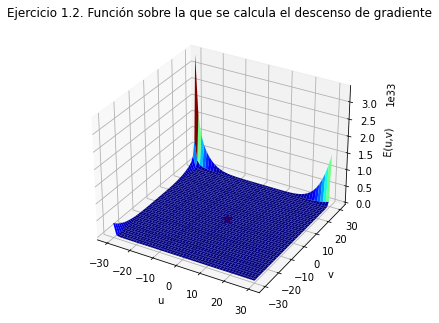
\includegraphics[width=0.65\textwidth]{images/plotE}
	\caption{Representación gráfica de $E$}
	\end{figure}
	
	Queremos encontrar valores $(u,v)$ que minimicen $E$. Para ello se ha implementado algoritmo \textit{Gradiente Descendiente} con tasa de aprendizaje $\eta = 0.1$ y punto inicial $(1,1)$, utilizaremos como condición de parada el encontrar un  $(\hat u,\hat v) \in \R^2$ con $E(\hat u, \hat v) < 10^{-14}$%, es decir acercarnos a valor que da 0 en $E$, que es el mínimo valor que toma $E$, con una precisión de $10^{-14}$
	
	\begin{itemize}
	\item	Calculamos las derivadas parciales de $E(u,v)=(u^3e^{v-2}-2v^2e^{-u})^2$
	$$\frac{\partial}{\partial u} E(u,v)=2(u^3e^{v-2}-2v^2e^{-u})(3u^2e^{v-2}+2v^2e^{-u})$$
	$$\frac{\partial}{\partial v} E(u,v)=2(u^3e^{v-2}-2v^2e^{-u})(u^3e^{v-2}-4e^{-u}v)$$
	quedándonos el gradiente
	$$\nabla E(u,v)=\begin{matrix}
	& \left(\begin{matrix}
	2(u^3e^{v-2}-2v^2e^{-u})(3u^2e^{v-2}+2v^2e^{-u})  \vspace{2.5mm}\\
	2(u^3e^{v-2}-2v^2e^{-u})(u^3e^{v-2}-4e^{-u}v)\\
	\end{matrix}\right)
	\end{matrix}
	$$
	\item El algoritmo ha tomado 10 iteraciones para obtener un $(\hat u,\hat v) \in \R^2$ con $E(\hat u, \hat v) < 10^{-14}$
	\item Las coordenadas $(\hat u, \hat v)$, en las que $E$ alcanzó por primera vez valor menor que $10^{-14}$, son $( 1.1572888496465497 , \ 0.9108383657484797 )$
	\end{itemize}
	\subsection{Apartado 3}
	Procedemos igual para $f\colon \R^2 \to \R$ con $f(x,y)=(x+2)^2+2(y-2)^2+2\sin(2\pi x)\sin(2\pi y)$, queremos encontrar valores que den valor mínimo en $f$.
	
	\begin{figure}[H]
	\centering
	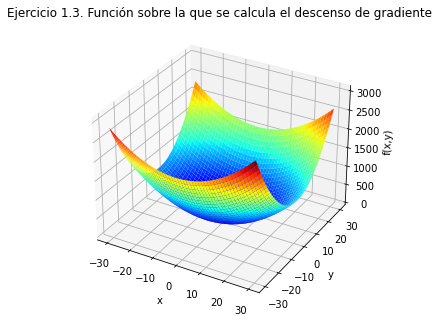
\includegraphics[width=0.65\textwidth]{images/plotF}
	\caption{Representación gráfica de $f$}
	\end{figure}
	
	Ahora utilizaremos punto inicial $(-1,1)$ y un máximo de 50 iteraciones. Veremos el comportamiento del algoritmo con las tasas de aprendizaje $\eta =0.01$ y $\eta = 0.1$, haremos una comparativa.
	\begin{itemize}
	\item Calculamos las derivadas parciales de $f(x,y)=(x+2)^2+2(y-2)^2+2\sin(2\pi x)\sin(2\pi y)$
	$$\frac{\partial}{\partial x} f(x,y)=2(x+2)+2cos(2\pi x)\sin(2\pi y)2\pi= 2(2\pi \cos(2\pi x)\sin(2\pi y)+x+2)$$
	$$\frac{\partial}{\partial y} f(x,y)=4(y-2)+2\sin(2\pi x)\cos(2\pi y)2\pi =4(\pi\sin(2\pi x)\cos(2\pi y)+y-2)$$
	quedándonos el gradiente
	$$\nabla f(x,y)=\begin{matrix}
	& \left(\begin{matrix}
	2(2\pi \cos(2\pi x)\sin(2\pi y)+x+2)  \vspace{2.5mm}\\
	4(\pi\sin(2\pi x)\cos(2\pi y)+y-2)\\
	\end{matrix}\right)
	\end{matrix}
	$$
	\item Veamos las gráficas que muestran los valores de $f(x,y)$ en función del número de iteraciones en el algoritmo para $\eta = 0.01$ y $\eta =0.1$
	
	\begin{figure}[H]
		\centering
		\begin{subfigure}{.5\textwidth}
  		\centering
  		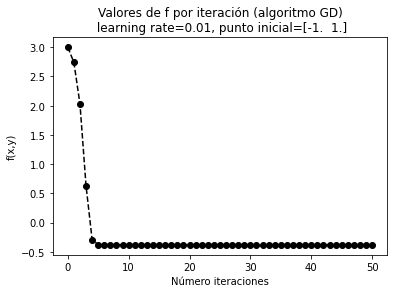
\includegraphics[width=1\textwidth]{images/f_por_iter_lr_01}
  		\caption{Tasa aprendizaje $\eta = 0.01$}
  		\label{fig:sub1}
		\end{subfigure}%
		\begin{subfigure}{.5\textwidth}
  		\centering
  		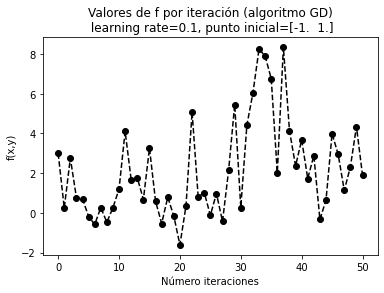
\includegraphics[width=1\textwidth]{images/f_por_iter_lr_1}
  		\caption{Tasa aprendizaje $\eta = 0.1$}
  		\label{fig:sub2}
		\end{subfigure}
		\caption{Valores de $f(x,y)$ en función del número de iteraciones}
		\label{fig:test}
	\end{figure}


	 
	 Podemos ver que, con tasa de aprendizaje $\eta = 0.01$, rápidamente disminuimos el valor de $f(x,y)$ en las primeras iteraciones, luego el valor de $f(x,y)$ llega un mínimo local y se estabiliza cerca de un valor cercano a $-0.5$, concretamente $-0.3812495$. Por otra parte, con tasa de aprendizaje $\eta = 0.1$, vemos que los valores de $f(x,y)$ van oscilando, no convergen a un mínimo local; lo que sí es destacable es que en la iteración 20 toma un valor cercano a $-2$, concretamente $-1.61701605$, en el punto $(-1.69871178, 1.80532287)$, sin embargo luego toma valores mayores que el tomado en la iteración 20.\\
	 
	 Pero... ¿Por qué se comporta así el algoritmo con $\eta =0.1$? ¿Por qué en la iteración 20 alcanza un valor menor si empieza en el mismo punto que con $\eta = 0.1$? ¿Por qué no sigue por el ``buen camino'' cuando estamos en la iteración 20 (o en las iteraciones anteriores que tomaba valores pequeños y luego mayores con el aumento de iteraciones)?\\
	 
	 Hay que recordar que $\eta$ influye proporcionalmente en cómo de grandes serán los pasos en la dirección ``más profunda''. El vector $-\nabla E_{in}(w)$, con sentido de mayor descenso, multiplicado por $\eta$ es lo que se suma al $w$ actual (en nuestro caso $w=(x,y)$), esto es, nos desplazamos en el espacio vectorial, $\R^2$, del dominio de la función. Es decir, con palabras informales; se toma ese vector  $-\nabla E_{in}(w)$ y nos desplazamos con él, multiplicado por cuánto quiero aprender $\eta$, a partir de $w$ actual para obtener el nuevo $w$. 
	 
	 Tasas de aprendizaje alto pueden hacer que el desplazamiento sea muy grande y nos ``saltemos'' la zona de mínimo local en la que estábamos. Esta sería la explicación para nuestro caso; la tasa de aprendizaje es muy alta y saltamos la zona de mínimo local en la que pudiéramos entrar, obteniendo así valores dispares (por saltar a una nueva zona), sin convergencia. Sin embargo con tasa de aprendizaje $\eta = 0.01$ sí entramos en zona de mínimo local, y converge al mismo, pues los pasos son lo suficientemente pequeños como para no saltar. 
	 
	 Podemos ver visualmente, con una imagen lo suficientemente ampliada, que efectivamente nuestra función tiene numerosas zonas con mínimos locales (se podía sospechar por los senos)
	 
	 \begin{figure}[H]
		\centering
		\begin{subfigure}{.5\textwidth}
  		\centering
  		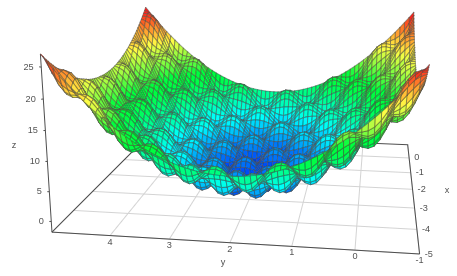
\includegraphics[width=1\textwidth]{images/repre_f}
  		%\caption{Tasa aprendizaje $\eta = 0.01$}
  		\label{fig:sub1}
		\end{subfigure}%
		\begin{subfigure}{.5\textwidth}
  		\centering
  		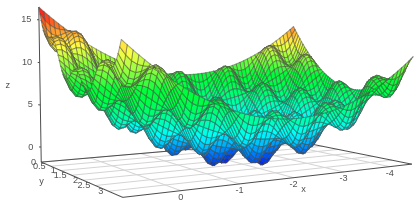
\includegraphics[width=1\textwidth]{images/repre_f_3}
  		%\caption{Tasa aprendizaje $\eta = 0.1$}
  		\label{fig:sub2}
		\end{subfigure}
		\caption{Representación de $f(x,y)$ ampliada, $z=f(x,y)$}
		\label{fig:test}
	\end{figure}
	 
	 En la iteración $20$ nuestro algoritmo con $\eta =0.1$ había encontrado una zona con un mínimo prometedor, pero lamentablemente tiene una tasa de aprendizaje muy alta y ``salta'' de la zona.
	 
	 \item Veamos una tabla, para distintos puntos de inicio, con los valores mínimos obtenidos en $f$ y los $(x,y)$ donde se alcanzan. Se han realizado 50 iteraciones en el algoritmo.
	 
	\begin{table}[htbp]
	\begin{center}
	\begin{tabular}{|c|c|c|}
	\hline
	Punto de inicio & Valor mínimo $f(x,y)$ & $(x,y)$ correspondiente al valor mínimo \\
	\hline \hline
	(-0.5, -0.5) & 9.125146662901855 & (-0.79349947, -0.12596576)\\ \hline
	(1, 1) & 6.4375695988659185 & (0.67743878, 1.29046913)\\ \hline
	(2.1, -2.1) & 12.490971442685035 & (0.14880583, -0.0960677)\\  \hline
	(-3, 3) & -0.38124949743809955 & (-2.73093565, 2.71327913)\\ \hline
	(-2, 2) & -4.799231304517944e-31 & (-2, 2)\\ \hline
	\end{tabular}
	\caption{Valor mínimo, tras 50 iteraciones, alcanzado por $f$ y punto donde se alcanza, en función del punto de inicio. \textit{Gradiente Descendente}.}
	\label{tabla:sencilla}
	\end{center}
	\end{table}
	
	En función del punto de inicio obtenemos un mejor o peor mínimo; por ejemplo, si comenzamos en $(-0.5, -0.5)$ obtenemos el mínimo $9.125\ldots$ (que ha sido el peor mínimo obtenido), mientras que comenzando el $(-3,3)$ obtenemos $-0.381\ldots$ (que ha sido el mejor mínimo obtenido).
	
	Podemos ver que, para los 4 primeros puntos iniciales hemos obtenido las gráficas
	\begin{figure}[H]
		\centering
		\begin{subfigure}{.5\textwidth}
  		\centering
  		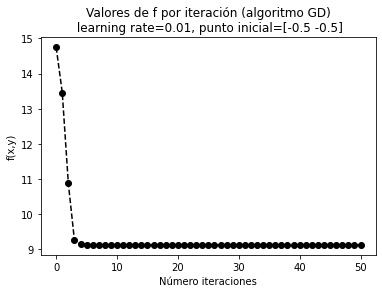
\includegraphics[width=1\textwidth]{images/1_3b_1}
  		%\caption{Punto de inicio $(-0.5, 0.5)$}
  		\label{fig:sub1}
		\end{subfigure}%
		\begin{subfigure}{.5\textwidth}
  		\centering
  		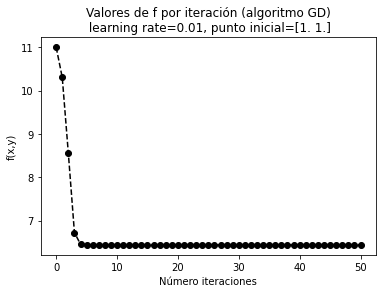
\includegraphics[width=1\textwidth]{images/1_3b_2}
  		%\caption{Punto de inicio $(1,1)$}
  		\label{fig:sub2}
		\end{subfigure}
		\caption{Valores de $f$ por iteración para puntos de inicio $(-0.5, -0.5)$ y $(1,1)$ respectivamente}
		\label{fig:test}
	\end{figure}
	
	\begin{figure}[H]
		\centering
		\begin{subfigure}{.5\textwidth}
  		\centering
  		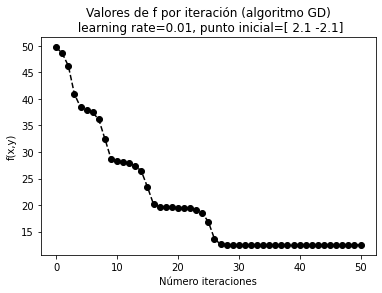
\includegraphics[width=1\textwidth]{images/1_3b_3}
  		%\caption{Punto de inicio $(2.1, -2.1)$}
  		\label{fig:sub1}
		\end{subfigure}%
		\begin{subfigure}{.5\textwidth}
  		\centering
  		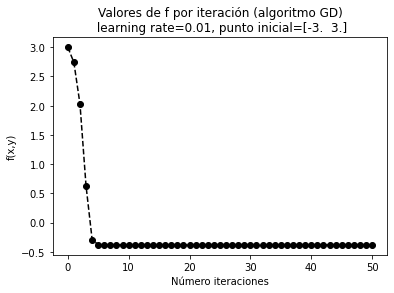
\includegraphics[width=1\textwidth]{images/1_3b_4}
  		%\caption{Punto de inicio $(-3,3)$}
  		\label{fig:sub2}
		\end{subfigure}
		\caption{Valores de $f$ por iteración para puntos de inicio $(2.1, -2.1)$ y $(-3,3)$ respectivamente}
		\label{fig:test}
	\end{figure}
	 hasta ahora, en todos los puntos iniciales, el algoritmo comienza con un valor alto de $f$ en su punto de inicio y va convergiendo hacia un mínimo.\\
	Cabe destacar el caso del punto de inicio $(-2,2)$
	
	\begin{figure}[H]
	\centering
	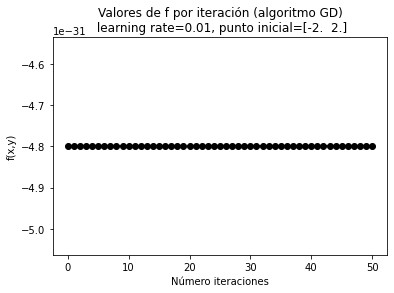
\includegraphics[width=0.55\textwidth]{images/1_3b_5}
	\caption{Valores de $f$ por iteración para punto de inicio $(-2,2)$}
	\end{figure}
	
	Se obtiene siempre el mismo valor, y es que no cambia del punto inicial, constantemente se evalúa en $(-2,2)$. Esto nos indica que estamos en un punto con gradiente nulo. Concretamente estamos ante un punto de silla, podemos visualizarlo gráficamente
	\iffalse
	\begin{figure}[H]
		\centering
		\begin{subfigure}{.5\textwidth}
  		\centering
  		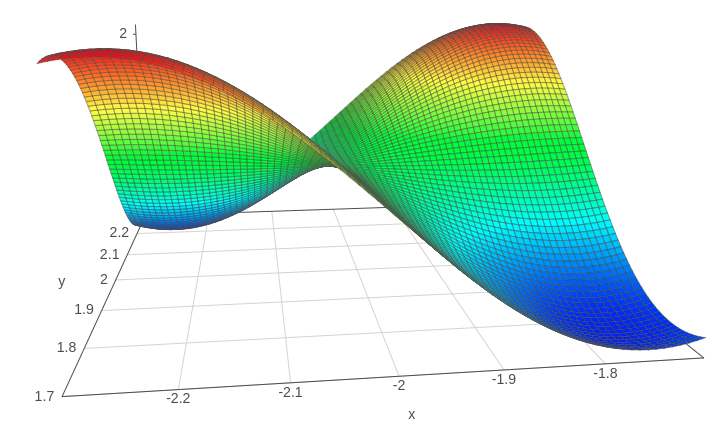
\includegraphics[width=1\textwidth]{images/punto_silla}
  		%\caption{Tasa aprendizaje $\eta = 0.01$}
  		\label{fig:sub1}
		\end{subfigure}%
		\begin{subfigure}{.5\textwidth}
  		\centering
  		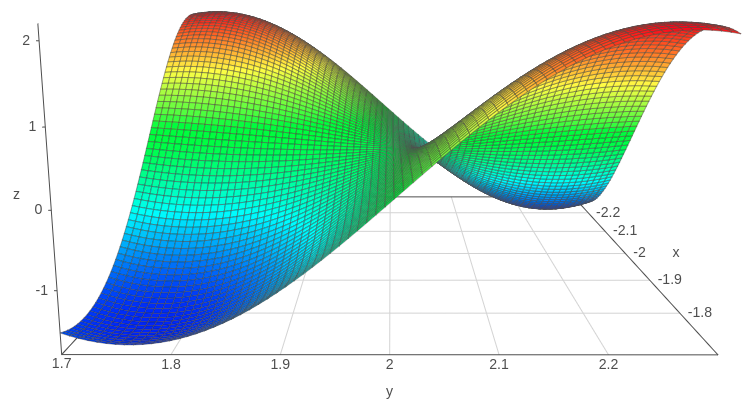
\includegraphics[width=1\textwidth]{images/punto_silla2}
  		%\caption{Tasa aprendizaje $\eta = 0.1$}
  		\label{fig:sub2}
		\end{subfigure}
		\caption{Dos imágenes del punto de silla en $(-2,2)$, $z=f(x,y)$}
		\label{fig:test}
	\end{figure}
	\fi
	
	\begin{figure}[H]
	\centering
	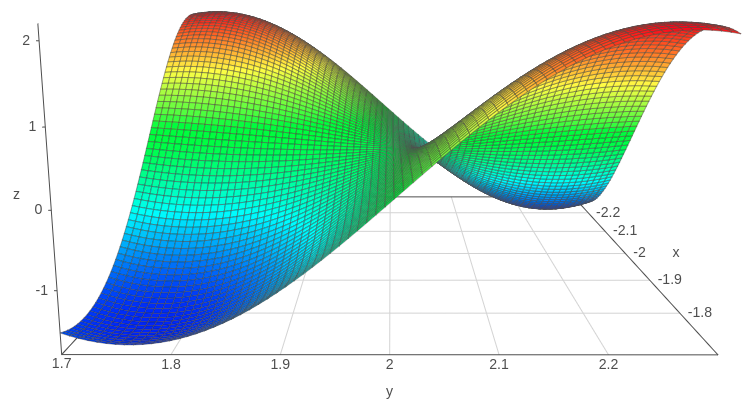
\includegraphics[width=0.55\textwidth]{images/punto_silla2}
	\caption{Imagen del punto de silla en $(-2,2)$, $z=f(x,y)$}
	\end{figure}	
	
	Al tener gradiente nulo en $(-2,2)$, \iffalse $-\eta \nabla f(x,y)$ evaluado en $(-2,2)$\fi $-\eta \nabla f(-2,2)$ es el vector nulo, y por tanto no hay desplazamiento del punto de inicio $(-2,2)$ en ninguna iteración.
	
	\end{itemize}	
	
	\subsection{Apartado 4}
	Después de los resultados obtenidos, podemos decir que hay dificultad en elegir 
	\begin{itemize} 
	\item Un buen punto inicial para nuestro problema. Hemos visto en el Apartado 3 que los mínimos obtenidos varían en función del punto inicial del que partimos. Dependiendo del punto inicial podemos caer en un mínimo local más o menos alejado del mínimo global.
	\item Una tasa de aprendizaje adecuada. Hemos visto en el Apartado 2 que una tasa de aprendizaje alta puede hacernos ``saltar'' de la zona de mínimo local. Una tasa de aprendizaje alta puede hacernos estar saltando mínimos locales sin estabilizarse en ninguno, y una tasa de aprendizaje baja puede hacernos caer y converger a mínimos locales que no nos interesan, aparte de que puede conllevar una convergencia muy lenta.
	\end{itemize}
	
	Además, en general, no conocemos el mínimo global de la función y por tanto tampoco si los mínimos que obtenemos están cerca de éste. En este caso, el cómo de bueno es un mínimo obtenido será relativo a los otros mínimos obtenidos.
	
	%\textit{Nota:} en el caso de que la función sea convexa tenemos la ventaja de que solo existe un mínimo, el global.
    \newpage
    \section{Ejercicio sobre Regresión Lineal.}
    
	\subsection{Apartado 1}
	
    \underline{\bf Algoritmo de la pseudo-inversa}\\
    
    $E_{in}$ puede expresarse en forma matricial
	$$E_{in}(w)=\frac{1}{N} \sum_{i=1}^N (w^Tx_i -y_i)^2=\frac{1}{N}\norm{Xw-y}^2$$
	donde
	$$
	X=\begin{matrix}
	& \left(\begin{matrix}
	- x_1^T - \\
	- x_2^T - \\
	...  \\
	- x_N^T - \\


	\end{matrix}\right)
	\end{matrix}
		\quad \quad 
	y=\begin{matrix}
	& \left(\begin{matrix}
	y_1 \\
	y_2 \\
	...  \\
	y_N  \\


	\end{matrix}\right)
	\end{matrix}
	$$
	
	Queremos minimizar
	$$E_{in}(w)=\frac{1}{N}\norm{Xw-y}^2=\frac{1}{N}(Xw-y)^T(Xw-y)=\frac{1}{N}((Xw)^TXw-y^TXw-(Xw)^Ty+y^Ty1)=$$ $$=\frac{1}{N} (w^TX^TXw-2w^TX^Ty+y^Ty)$$
	es decir, buscamos vector de pesos $w_{lin} \in \R^{d+1}$ con $E_{in}(w_{lin})=\min_{w\in \R^{d+1}} E_{in}(w)$. Para minimizar $E_{in}$ igualamos gradiente a 0
	$$\nabla E_{in}(w)=\frac{2}{N} X^T (Xw-y)=2X^TXw-2X^Ty=0$$
	y queda
	$$X^TXw= X^Ty$$
	que se reescribe como
	$$w=X^\dagger y \quad \text{ donde } \quad X^\dagger :=(X^TX)^{-1}X^T \ \ \text{ (pseudo-inversa de } X\text{)}$$
	$\Rightarrow w_{lin}=X^\dagger y$.
	Por tanto, dados $X$ e $y$, el algoritmo consiste en calcular $X^\dagger =(X^TX)^{-1}X^T$ y devolver $w_{lin}=X^\dagger y$
	
	Para calcular $(X^TX)^{-1}$ se puede usar la descomposición en valores singulares (SVD), $X=UDV^T$, y queda $(X^TX)^{-1}=VD^*V^T$ (si $D$ tiene $e_0,\ldots,e_d$ como elementos de la diagonal, la matriz $D^*$ tiene, en la diagonal, $\frac{1}{e_i^2}$ como elementos o $0$ si $e_i=0$) \\
	
	\textit{Nota:} Una desventaja de este método es que el cálculo matricial hace que no sea un método con buena escalabilidad, grandes cantidades de datos pueden dar lugar a matrices no abordables. \\

	\underline{\bf Gradiente Descendente Estocástico}\\
	
	Este método, a diferencia de \textit{Gradiente Descendente}, trabaja con minibatches (pequeñas submuestras de la muestra). Está comprobado empíricamente que el uso de estos minibatches para el cálculo del gradiente mejora el óptimo obtenido para funciones no convexas. Al trabajar con submuestra pequeña es probable que en los pasos o desplazamientos del algoritmo se evite caer en mínimos locales no deseables (valor alto), mínimos locales en los que sí se entraría si trabajasemos con toda la muestra.

	\iffalse Una vez que está definido el vector que usaremos para desplazarnos en busca de un mínimo, podemos describir el proceder del algoritmo.\fi Se toma una tasa de aprendizaje $\eta$, un punto inicial $w=w_0\in \text{Dominio}(E_{in})$. Se divide la muestra en una secuencia de minibatches aleatorios. Iteramos los minibatches y en base a cada minibatch, $minibatch \in Minibatches$, se actualiza el valor de $w$
	$$w:=w-\eta \nabla E_{in}^{minibatch}(w)$$
	repetimos esta división en minibatches y los cálculos de $w$ por cada $minibatch \in Minibatches$ \iffalse esta toma de minibatch y cálculo de $w$ en función del minibatch\fi hasta una condición de parada, ya sea por iteraciones o por encontrar un valor suficientemente pequeño para $E_{in}$\\
	
	
	Las implementaciones (autoexplicativas) para método Pseudoinversa y SGD realizadas son
		\begin{lstlisting}[language=Python, caption= Implementaci\'on del m\'etodo por Pseudoinversa en Python, inputencoding=latin1]
  # Pseudoinversa	
'''
   Implementación de método por pseudoinversa.
   
   :param numpy.ndarray X: matriz muestral de vectores de características
   :param numpy.ndarray y: etiquetas o clases de la muestra
   :return: el vector de pesos que minimiza el ECM para la muestra
'''
def pseudoinverse(X, y):
    # Descomposición por valores singulares
    U, d, Vt = np.linalg.svd(X) 
    # Construimos la matriz D_, matriz que en su diagonal tiene 1 entre el cuadrado de cada valor singular o 0 si el valor singular es 0
    d = np.array([np.inf if i == 0 else i for i in d]) # cambiamos los ceros por np.inf (para dividir después y obtener D_)
    d = 1 / (d*d)
    D_ = np.diag(d)
    # Devolvemos el producto de la pseudoinversa por y, (es decir el vector de pesos que minimiza el ECM para la muestra)
    return ((((V.T).dot(D_)).dot(V)).dot(X.T)).dot(y)
	\end{lstlisting}
	
			\begin{lstlisting}[language=Python, caption= Implementaci\'on del m\'etodo por SGD en Python, inputencoding=latin1]
  # Gradiente Descendente Estocastico
'''
   Implementación de algoritmo Gradiente Descendente Estocástico. (condición de parada por iteraciones)
   
   :param numpy.ndarray X: matriz muestral de vectores de características
   :param numpy.ndarray y: etiquetas o clases de la muestra
   :param numpy.ndarray w0: vector de pesos inicial
   :param learning_rate: tasa de aprendizaje para GDE
   :param max_iter: iteraciones máximas en GDE
   :return: el último vector de pesos calculado
'''
def sgd(X, y, w0, learning_rate, minibatches_size, max_iterations):
    w = w0 
    sample_size = X.shape[0] # tamaño de muestra
    indexes = np.arange(sample_size) # trabajaremos con índices
    # Mezclamos aleatoriamente la muestra (trabajando con índices) por primera vez
    np.random.shuffle(indexes)
    # Marcamos el primer minibatch
    minibatch_init = 0
    minibatch_end = minibatch_init + minibatches_size
    
    # Hasta que no alcancemos el máximo de iteraciones
    for i in range(max_iterations):
        # Si ya hemos iterado en todos los minibatches
        if (minibatch_init > sample_size):
            # Mezclamos aleatoriamente muestra (trabajando con índices), generando así nuevos minibatches
            np.random.shuffle(indexes)
            # reestablecemos valores para empezar por primer minibatch
            minibatch_init = 0
            minibatch_end = minibatch_init + minibatches_size
        
        # Se toma el minibatch actual
        minibatch = indexes[minibatch_init:minibatch_end]
        # Se calcula el vector pesos para el minibatch tomado (dando el 'paso de mayor profundidad' en el minibatch)
        w = w - learning_rate * grad_Ein_minibatch(X[minibatch], y[minibatch], w)
        # Se avanza al siguiente minibatch
        minibatch_init += minibatches_size
        minibatch_end += minibatches_size
        
    return w
	\end{lstlisting}~\\
	
	Resultados obtenidos:
	\begin{itemize}
		\item Por el método \textit{SGD}, después de 1000 iteraciones, hemos obtenido vector de pesos $\hat w=(-1.24069346, -0.17997056, -0.46016084)$. Distintos valores para vector de pesos inicial, tasa de aprendizaje o tamaño minibatches ofrecían más o menos error $E_{in}$ y $E_{out}$. Para obtener $\hat w$ se ha utilizado una tasa de aprendizaje $0.01$, vector de pesos inicial $(0,0,0)$ y minibatches de tamaño 32. \\
		Podemos visualizar la regresión obtenida gráficamente
		\begin{figure}[H]
		\centering
		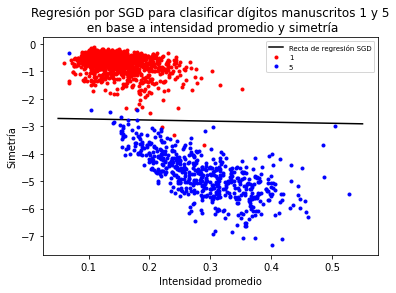
\includegraphics[width=0.6\textwidth]{images/regre_SGD}
		\caption{Regresión obtenida mediante \textit{SGD}}
		\end{figure}
	
	\item Por el método de Pseudoinversa se ha obtenido el vector de pesos $w_{lin}=(-1.11588016,\\-1.24859546,-0.49753165)$, que es donde $E_{in}$ alcanza el mínimo valor.\\
	Podemos visualizar la regresión obtenida gráficamente
		\begin{figure}[H]
		\centering
		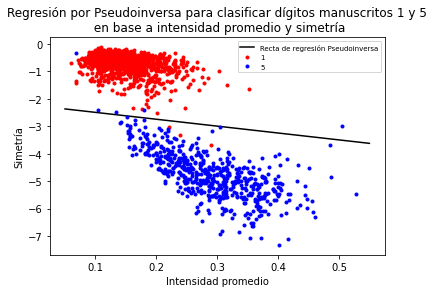
\includegraphics[width=0.63\textwidth]{images/regre_Pseudo}
		\caption{Regresión obtenida mediante Pseudoinversa}
		\end{figure}
	\end{itemize}
	
	Una gráfica conjunta comparativa
	\begin{figure}[H]
		\centering
		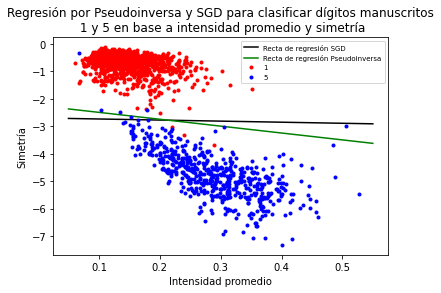
\includegraphics[width=0.63\textwidth]{images/regre_comparativa}
		\caption{Regresión mediante Pseudoinversa y \textit{SGD}}
		\end{figure}
 Podemos ver una tabla comparativa de los errores dentro y fuera de la muestra obtenidos con ambos métodos.
	
	\begin{table}[htbp]
	\begin{center}
	\begin{tabular}{|c|c|c|}
	\hline
	Método & $E_{in}$ & $E_{out}$ \\
	\hline \hline
	SGD & 0.0816898877496507 & 0.13581861169470588\\ \hline
	Pseudoinversa & 0.07918658628900395 & 0.13095383720052586\\ \hline
	\end{tabular}
	\caption{Errores dentro y fuera de la muestra para regresión por SGD y Pseudoinversa.}
	\label{tabla:sencilla}
	\end{center}
	\end{table}
	
	Observando la tabla comparativa podemos comprobar que el método por Pseudoinversa ofrece mejor resultado para minimizar $E_{in}$. Esto era esperable pues el método por Pseudoinversa ofrece el mínimo global (hay que recordar que estamos trabajando con $E_{in}$ que es una función convexa y por tanto tiene mínimo global), mientras que mediante \textit{SGD} lo que obtenemos son aproximaciones del mínimo global. Además este mínimo global ofrecido por el método de Pseudoinversa, $E_{in}(w_{lin})$, coincide con el error fuera de la muestra, $E_{out}(w_{lin})$, cuando el tamaño de la muestra, $N$, diverge, $N\to \infty$; siempre es preferible trabajar con Pseudoinversa directamente (si el tamaño de la muestra lo permite) en vez de con las aproximaciones ofrecidas por $\textit{SGD}$.
	
	 Aún así, mediante \textit{SGD} obtenemos una buena solución, aunque para obtenerla hay que ajustar bien los parámetros, como elegir bien el número de iteraciones, la tasa de aprendizaje y el tamaño de los minibatches. 
	
	%También podemos observar que mediante Pseudoinversa obtenemos también menor error, $E_{out}$, fuera de la muestra. Esto también era esperable pues sabemos que el error dentro de la muestra, $E_{in}$, coincide con el error fuera de la muestra, $E_{out}$, cuando el tamaño de la muestra, $N$, diverge, $N\to \infty$.
	
	\subsection{Apartado 2}
	Generamos la muestra de 1000 puntos en el cuadrado $[-1,1]\times [-1,1]$
	\begin{figure}[H]
		\centering
		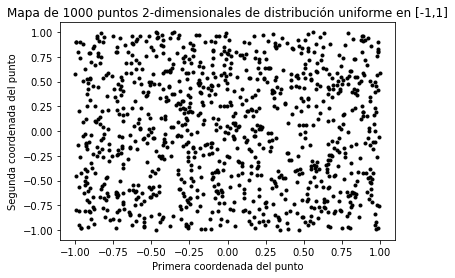
\includegraphics[width=0.63\textwidth]{images/dist_unif_puntos}
		\caption{1000 puntos bidimensionales siguiendo distribución uniforme en $[-1,1]$}
	\end{figure}
	
	Después de clasificar mediante la función $f(x_1,x_2)=sign((x_1 - 0.2)^2 + x_2^2 - 0.6)$, tenemos la gráfica
	
	\begin{figure}[H]
		\centering
		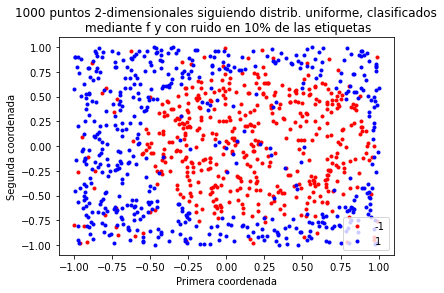
\includegraphics[width=0.65\textwidth]{images/1000_puntos_unif_clasi}
		\caption{Puntos anteriormente generados clasificados mediante $f$ y con ruido en 10\% de las etiquetas}
	\end{figure}
	
	Hacemos regresión por el método de Pseudoinversa y obtenemos $w_{lin}= (0.04675207, \\-0.4425426, -0.02202655)$ con $E_{in}(w_{lin})=0.9321294905907557$. Mediante \textit{SGD}, con tasa de aprendizaje $0.01$, tamaño minibatches 32, punto inicial $(0,0,0)$ y 1000 iteraciones, obtenemos $\hat w = (0.0425056, -0.43326552, -0.0312279)$ con $E_{in}(\hat w)=0.9322063797449904$. Por ambos métodos obtenemos prácticamente los mismos errores dentro de la muestra. Los errores son altos, podemos visualizar gráficamente las rectas obtenidas
	\iffalse
	\begin{figure}[H]
		\centering
		\begin{subfigure}{.488\textwidth}
  		\centering
  		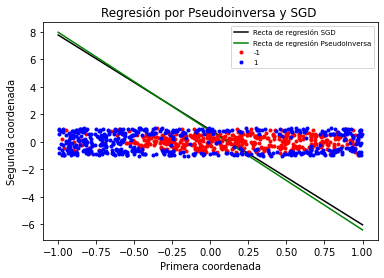
\includegraphics[width=1\textwidth]{images/2_3_c}
  		%\caption{Tasa aprendizaje $\eta = 0.01$}
  		\label{fig:sub1}
		\end{subfigure}%
		\begin{subfigure}{.512\textwidth}
  		\centering
  		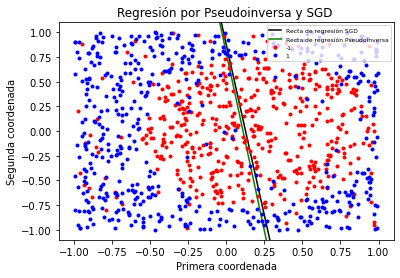
\includegraphics[width=1\textwidth]{images/2_3_c2}
  		%\caption{Tasa aprendizaje $\eta = 0.1$}
  		\label{fig:sub2}
		\end{subfigure}
		\caption{Rectas regresión obtenidas mediante método Pseudoinversa y \textit{SGD}}
		\label{fig:test}
	\end{figure}
	\fi
	\begin{figure}[H]
		\centering
		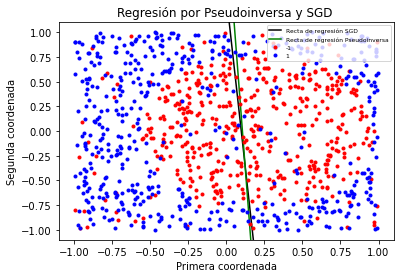
\includegraphics[width=0.65\textwidth]{images/2_3_c_bueno}
		\caption{Rectas regresión obtenidas mediante método Pseudoinversa y \textit{SGD}}
	\end{figure}
	
	Las aproximaciones a $f$ no son buenas, esto se debe a que estamos intentando ajustar puntos cuyas etiquetas, -1 y 1, dadas por $f$, dan lugar a dos conjuntos, nube de puntos roja y azul, difícilmente separables por una recta. También se podía sospechar ya que estamos intentando aproximar linealmente a $f$, que no tiene naturaleza lineal.
	
	Veamos una tabla comparativa del promedio de errores, dentro y fuera de la muestra, de 1000 muestras con 1000 puntos cada una
	%Veamos una tabla comparativa de la media de errores dentro y fuera de la muestra después de 1000 iteraciones\\
	
	\begin{table}[htbp]
	\begin{center}
	\begin{tabular}{|c|c|c|}
	\hline
	Método & $E_{in}$ & $E_{out}$ \\
	\hline \hline
	SGD & 0.9274471985970024 & 0.9324717807833176\\ \hline
	Pseudoinversa & 0.9273163854093703 & 0.9324170083670043\\ \hline
	\end{tabular}
	\caption{Errores promedio dentro y fuera de la muestra para regresión por SGD y Pseudoinversa, 1000 muestras.}
	\label{tabla:sencilla}
	\end{center}
	\end{table}
	
	Mediante el método de Pseudoinversa obtenemos mejores resultados, mientras el tamaño de la muestra nos lo permita este método siempre nos dará el mejor ajuste para minimizar $E_{in}$. La diferencia de errores con \textit{SGD} no es muy significativa.\\
	
	Ahora utilizaremos el vector de características $(1,x_1,x_2,x_1x_2,x_1^2,x_2^2)$. El vector de pesos obtenido mediante método de Pseudoinversa es $w_{lin}=(-0.88093471, -0.51092622,  -0.03471847,\\ -0.12182019,  1.18231995,  1.56403309)$ con $E_{in}(w_{lin})=0.5718308272094729$, el obtenido mediante \textit{SGD} es $\hat w=(-0.66077998, -0.50326448, -0.04740595, -0.12211729,  0.90810351,  1.23301988)$ con $E_{in}(\hat w)=0.5892224518277474$. Los errores dentro de la muestra se han reducido considerablemente respecto al modelo anterior. Podemos visualizar gráficamente la regresión realizada
	\begin{figure}[H]
		\centering
		\begin{subfigure}{.488\textwidth}
  		\centering
  		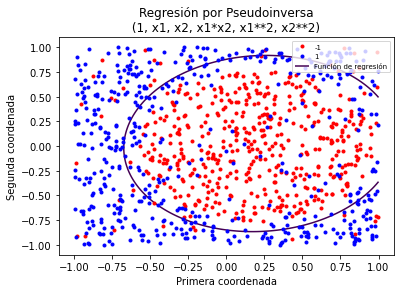
\includegraphics[width=1\textwidth]{images/elip_pseudo}
  		%\caption{Tasa aprendizaje $\eta = 0.01$}
  		\label{fig:sub1}
		\end{subfigure}%
		\begin{subfigure}{.512\textwidth}
  		\centering
  		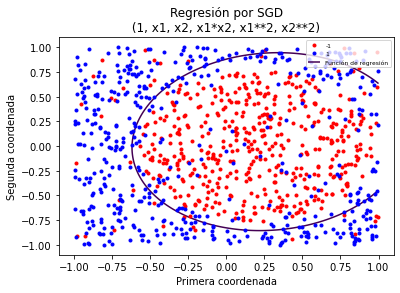
\includegraphics[width=1\textwidth]{images/elip_sgd}
  		%\caption{Tasa aprendizaje $\eta = 0.1$}
  		\label{fig:sub2}
		\end{subfigure}
		\caption{Elipses de regresión obtenidas mediante método Pseudoinversa y \textit{SGD}}
		\label{fig:test}
	\end{figure}
	
	Veamos, de nuevo, una tabla comparativa del promedio de errores, dentro y fuera de la muestra, de 1000 muestras con 1000 puntos cada una
	\begin{table}[htbp]
	\begin{center}
	\begin{tabular}{|c|c|c|}
	\hline
	Método & $E_{in}$ & $E_{out}$ \\
	\hline \hline
	SGD & 0.5992165370555411 & 0.6051599481381328\\ \hline
	Pseudoinversa & 0.5799894199671453 & 0.5864016468421366\\ \hline
	\end{tabular}
	\caption{Errores promedio dentro y fuera de la muestra para regresión, con nuevo vector de características, por SGD y Pseudoinversa, 1000 muestras.}
	\label{tabla:sencilla}
	\end{center}
	\end{table}
	
	Mediante este modelo, con vector de características $(1,x_1,x_2,x_1x_2,x_1^2,x_2^2)$, obtenemos menor error dentro y fuera de la muestra tanto para el método de Pseudoinversa como \textit{SGD}. Como la idea de hacer regresión es predecir etiquetas para nuevas entradas muestrales (nuevos vectores de características), lo que nos importa es el error fuera de la muestra; por tanto es más adecuado este segundo modelo, con vector de características $(1,x_1,x_2,x_1x_2,x_1^2,x_2^2)$, que ofrece menor error fuera de la muestra.
	
	\section{Ejercicio Bonus.}
	\underline{\bf Método de Newton}\\
	
		Éste método se utiliza cuando se está muy cerca de un óptimo porque ya se haya avanzado con algún método, \textit{Gradiente Descendente} por ejemplo, y se ve que los valores de las derivadas ya no son valores muy grandes. En ese caso estamos cerca del óptimo local que vamos a conseguir. Se podría seguir iterando..., la alternativa que ofrece este método es hacer una aproximación al óptimo suponiendo una superficie en paraboloide (buscar óptimo del paraboloide y suponer que ese óptimo es nuestro óptimo).\\
	
	A diferencia de \textit{Gradiente Descendente}, utilizaremos desarrollo Taylor de 2do orden (2do orden nos aporta aproximación de la curvatura en un entorno). Denotamos por $H_{E_{in}}$ a la matriz \textit{Hessiana} de $E_{in}$
	\begin{itemize}	
	\item Supongamos que ya estamos en un $w_0$ bueno (está cerca del óptimo). Vamos a ver si se puede calcular un incremento $\Delta w$ para que $w_0+ \Delta w$ sea el valor que nos da el óptimo
	$$g(\Delta w)=E_{in}(w_0+\Delta w) \stackrel{Taylor}{\approx} E_{in}(w_0)+\Delta w^T\nabla E_{in}(w_0)+\frac{1}{2} \Delta w^T \nabla ^2 E_{in} (w_0)\Delta w$$
	Ahora imponemos $\frac{\partial g(\Delta w)}{\partial\Delta w}=0$ (queremos llegar al mínimo, notar que se impondrá sobre la aproximación), y como 
	$$\frac{\partial}{\partial \Delta w} \left( \frac{1}{2} \Delta w^T \nabla ^2 E_{in} (w_0)\Delta w \right) = \frac{1}{2} \underbrace{\left( \nabla ^2 E_{in}(w_0) + (\nabla ^2 
E_{in}(w_0))^T\right)}_{ 2 \nabla ^2 E_{in}(w_0) } \Delta w  $$  
	(en las última llave se utiliza la conmutatividad de derivadas parciales por \textit{Teorema de Schwartz}), queda
	$$\nabla E_{in}(w_0)+\underbrace{\nabla^2 E_{in}(w_0)}_{H_{E_{in}}(w_0)} \Delta w=0$$
si $H_{E_{in}}(w_0)$ es definida positiva entonces la evaluación de $w_0 + \Delta w$, en la aproximación cuadrática (la que nos da el desarrollo de Taylor de 2do orden), da un mínimo local en la aproximación, y podemos determinar el paso necesario, $\Delta w$, para obtener el valor, $w_0+\Delta w$, que minimiza a la aproximación
	$$\Delta w=-H_{E_{in}}(w_0)^{-1} \nabla E_{in} (w_0)$$
	Si partíamos de un $w_0$ suficientemente próximo de un punto que da mínimo de $E_{in}$, nos dará una buena aproximación del punto que da ese mínimo de $E_{in}$ (esto es importante, puede ayudar a curar la oscilación)
	
	Después se puede tomar $w_0=w_0 +\Delta w$, y repetir el proceso. Es un método iterativo.
	\end{itemize}
	Notas:
	
	\begin{itemize}
		\item No se determina $\eta$ como en el método \textit{Gradiente Descendente}, este método directamente determina la dirección y el tamaño del paso.
	
		\item Este método debe de utilizarse cuando se está cerca del óptimo (la información sobre la curvatura en $E_{in}(w_0)$ dada por $H_{E_{in}}(w_0)$ es local, si no estamos lo suficientemente próximos podría ser  $H_{E_{in}}(w_0)$ definida negativa por ejemplo, y no estaríamos yendo al mínimo)
	
		\item Es útil cambiar a este método cuando estamos cerca del óptimo. Podemos llegar al óptimo en un número finito de pasos, curando la oscilación.
	
		\item El tener que calcular la matriz $H_{E_{in}}^{-1}$ hace que no sea el método idóneo cuando tenemos muchos datos. Para tamaños pequeños sí funciona bien.
	\end{itemize} ~\\
	
	Recordamos que $f(x,y)=(x+2)^2+2(y-2)^2+2\sin(2\pi x)\sin(2\pi y)$. Podemos calcular analíticamente la matriz \textit{Hessiana} de $f$, $H_f$
	$$H_f=\begin{matrix}
	 \left(\begin{matrix}
	2-8\pi ^2 \sin(2\pi x)\sin(2\pi y) & 8\pi^2\cos(2\pi x)\cos(2\pi y)\\
	8\pi ^2 \cos(2\pi x)\cos(2\pi y) & 4-8\pi ^2\sin(2\pi x)\sin(2\pi y)\\
	\end{matrix}\right)
	\end{matrix}
	$$
	
		Código del algoritmo implementado en Python (autoexplicativo)
	
	\begin{lstlisting}[language=Python, caption= Implementaci\'on del M\'etodo de Newton en Python, inputencoding=latin1]
   '''
   Método de Newton.
   
   :param np.array gradf: gradiente de la función a minimizar
   :param np.array Hessiana_f: matriz hessiana de la función a minimizar
   :param np.array initial_point: punto inicial, (se supone cerca de un mínimo)
   :param int max_iter: iteraciones del algoritmo
   :return: el punto del mínimo aproximado tras max_iter iteraciones
'''
def met_newton_f(gradf, Hessiana_f, initial_point, max_iter):
    w_actual = initial_point
    # Repetimos max_iter veces
    for i in range(max_iter):
        # Calculamos la inversa de la Hessiana de f evaluada en w_actual
        Hessiana_inv = np.linalg.inv(Hessiana_f(w_actual[0], w_actual[1]))
        # El nuevo punto es el actual - el producto de la Hessiana de f evaluada en w_actual por el gradiente de f evaluado en w_actual
        w_actual = w_actual - Hessiana_inv.dot(gradf(w_actual[0], w_actual[1]))
        
    return w_actual    
	\end{lstlisting}
	
	Veamos una tabla, para distintos puntos de inicio, con los valores mínimos obtenidos en $f$ y los $(x,y)$ donde se alcanzan. Se han realizado 50 iteraciones en el algoritmo.
	 
	\begin{table}[htbp]
	\begin{center}
	\begin{tabular}{|c|c|c|}
	\hline
	Punto de inicio & Último valor $f(x,y)$ & Último valor $(x,y)$ \\
	\hline \hline
	(-0.5, -0.5) & 7897.582180054467 & (41.07863112, -52.96175024)\\ \hline
	(1, 1) & 11.344755748360596 & (1.06737264, 0.91007092)\\ \hline
	(2.1, -2.1) & 96.54631298064457 & (3.82834647, -3.65961919)\\  \hline
	(-3, 3) & 3.1079800610352026 & (-3.05397555, 3.02846146)\\ \hline
	(-2, 2) & -4.799231304517944e-31 & (-2, 2)\\ \hline
	\end{tabular}
	\caption{Valor mínimo, tras 50 iteraciones, alcanzado por $f$ y punto donde se alcanza, en función del punto de inicio. Método de Newton.}
	\label{tabla:sencilla}
	\end{center}
	\end{table}
	
	Como se puede observar, excepto para el punto $(-2,2)$, en el que ya sabemos que hay un punto de silla, obtenemos valores mucho más altos que mediante  \textit{Gradiente Descendiente} (ver Cuadro 1). 
	
	Veamos gráficamente, para los distintos puntos iniciales, los valores de $f$ que se van tomando por iteración
	\begin{figure}[H]
		\centering
		\begin{subfigure}{.5\textwidth}
  		\centering
  		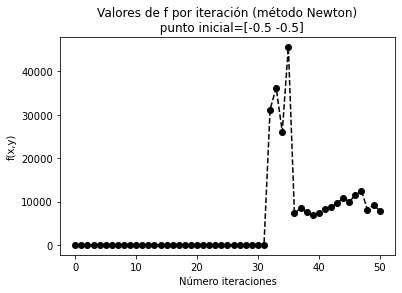
\includegraphics[width=1\textwidth]{images/newton1}
  		%\caption{Punto de inicio $(-0.5, 0.5)$}
  		\label{fig:sub1}
		\end{subfigure}%
		\begin{subfigure}{.5\textwidth}
  		\centering
  		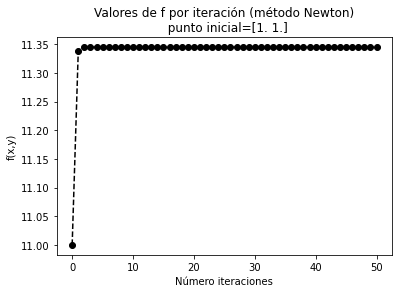
\includegraphics[width=1\textwidth]{images/newton2}
  		%\caption{Punto de inicio $(1,1)$}
  		\label{fig:sub2}
		\end{subfigure}
		\caption{Valores de $f$ por iteración para puntos de inicio $(-0.5, -0.5)$ y $(1,1)$ respectivamente}
		\label{fig:test}
	\end{figure}
	
	\begin{figure}[H]
		\centering
		\begin{subfigure}{.5\textwidth}
  		\centering
  		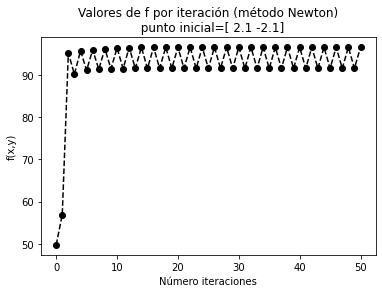
\includegraphics[width=1\textwidth]{images/newton3}
  		%\caption{Punto de inicio $(2.1, -2.1)$}
  		\label{fig:sub1}
		\end{subfigure}%
		\begin{subfigure}{.5\textwidth}
  		\centering
  		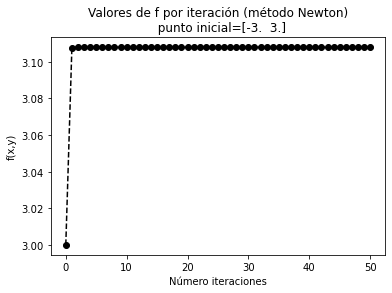
\includegraphics[width=1\textwidth]{images/newton4}
  		%\caption{Punto de inicio $(-3,3)$}
  		\label{fig:sub2}
		\end{subfigure}
		\caption{Valores de $f$ por iteración para puntos de inicio $(2.1, -2.1)$ y $(-3,3)$ respectivamente}
		\label{fig:test}
	\end{figure}
	\begin{figure}[H]
	\centering
	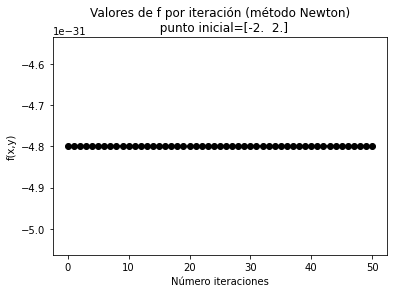
\includegraphics[width=0.55\textwidth]{images/newton5}
	\caption{Valores de $f$ por iteración para punto de inicio $(-2,2)$}
	\end{figure}
	
	Vemos que a diferencia de \textit{Gradiente Descendente} aquí no hay una sucesión decreciente de los valores de $f$ por iteración. \\
	En los puntos iniciales $(1,1)$ y $(-3,3)$ se estabiliza en punto con gradiente 0. No hay que olvidar que nuestra función $f$ está repleta de este tipo de puntos (ver Figura 4). En $(2.1, -2.1)$ va a zona con valores en $f$ más altos y luego va saltando, oscila, entre dos puntos. En $(-2,2)$ ya sabemos que hay un punto de silla. Por último, en $(-0.5,-0.5)$ pareciese que estuviese estable en las primeras 30 iteraciones pero podemos ver que no,
	\begin{figure}[H]
	\centering
	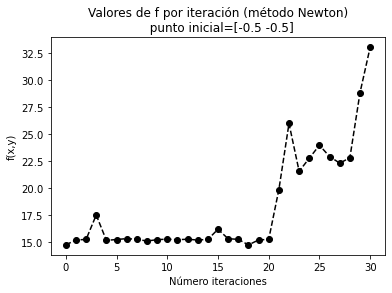
\includegraphics[width=0.55\textwidth]{images/newton6}
	\caption{Valores de $f$ por iteración para punto de inicio $(-0.5,0.5)$}
	\end{figure}
	no hay ningún tipo de convergencia.\\
	
	Los resultados no son nada parecidos a los obtenidos con \textit{Gradiente Descendiente} (ver figuras 5 y 6). La explicación de la no convergencia es deducible de la propia introducción teórica del método. La idea es aproximar la curvatura, por desarrollo de Taylor de 2do orden, \underline{muy cerca de un mínimo} para así aproximar el mínimo. Sin embargo, para los puntos iniciales usados no tenemos información de que estén cerca de un mínimo, no se ha utilizado ningún método, como \textit{Gradiente Descendente} por ejemplo, hasta la obtención de los mismos.\\
	Es importante estar lo suficientemente cerca de un mínimo. Para funciones de una variable se puede ilustrar este hecho de forma sencilla. Supongamos que queremos llegar al mínimo local $\sin(\frac{3\pi}{2})$, $\frac{3\pi}{2} \approx 4.7124$, veremos la situación para distintos puntos iniciales. En línea roja se visualiza la aproximación de Taylor de 2do orden\\ ~\\
	
	\begin{figure}[H]
		\centering
		\begin{subfigure}{.5\textwidth}
  		\centering
  		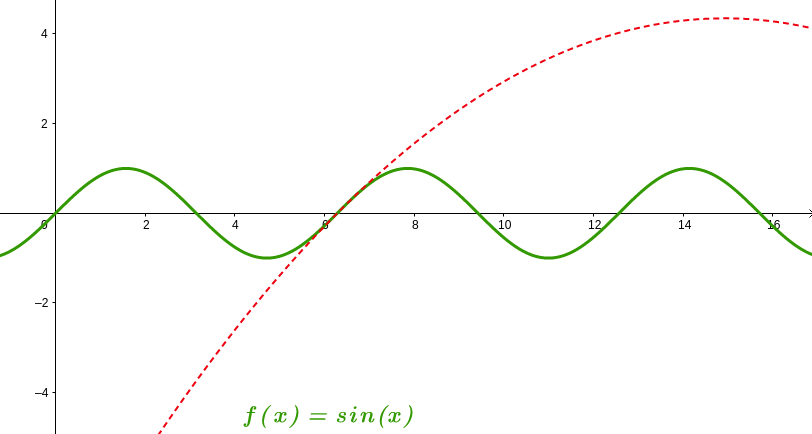
\includegraphics[width=0.95\textwidth]{images/ilus_newton1}
  		\caption{Aproximación Taylor para punto demasiado alejado del mínimo. Si fuese superficie tendría Hessiana negativa (no iríamos al mínimo). El punto con derivada 0 de la aproximación está ``muy a la derecha'', nos desplazaría a zona de la función muy alejada.}
  		\label{fig:f2}
		\end{subfigure}%
		\begin{subfigure}{.5\textwidth}
  		\centering
  		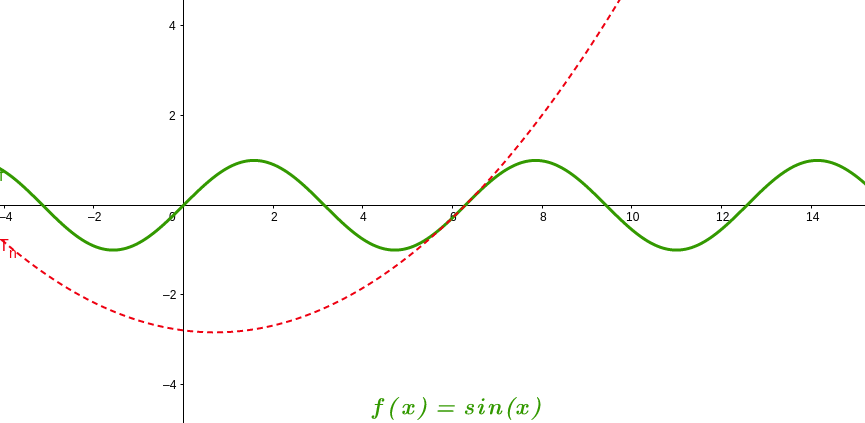
\includegraphics[width=0.95\textwidth]{images/ilus_newton2}
  		\caption{Aproximación Taylor para punto alejado del mínimo. Al menos ahora la aproximación es convexa, pero el punto con derivada 0 de la aproximación nos desplazaría muy a la izquierda, fuera de la zona del mínimo en $\frac{3\pi}{2}$}
  		\label{fig:f1}
		\end{subfigure}
		%\caption{Aproximaciones de Taylor de $\sin(x)$ con distintos puntos iniciales. Se busca el mínimo en $\frac{3\pi}{2} \approx 4.7124$}
		\label{fig:test}	
	\end{figure}
	\newpage
	\begin{figure}[H]
	\ContinuedFloat
	\centering
	\begin{subfigure}{\textwidth}
		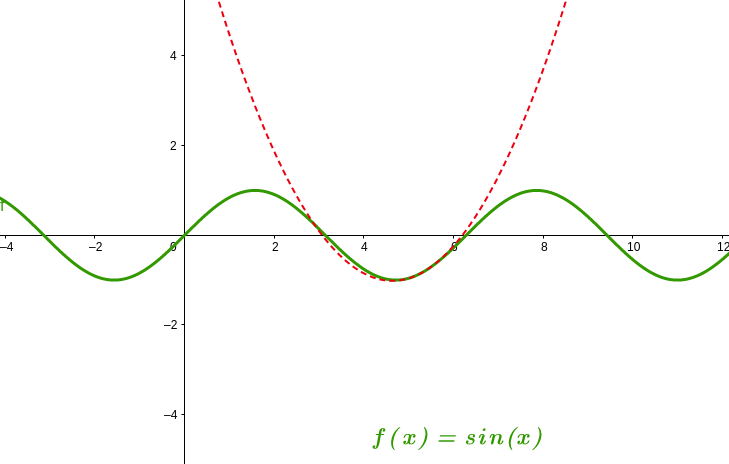
\includegraphics[width=0.55\textwidth]{images/ilus_newton3}
		\caption{Aproximación de Taylor para punto lo suficientemente cercano. El punto con derivada 0, de la aproximación de Taylor de 2do orden, es una buena estimación del mínimo local. Aquí sí nos daría un buen resultado el método de Newton. }
	\end{subfigure}
	\caption{Aproximaciones de Taylor de $\sin(x)$ con distintos puntos iniciales. Se busca el mínimo en $\frac{3\pi}{2} \approx 4.7124$}
	\end{figure}
	
	Lo que ha ocurrido, en la repetición del experimento, es que no se estaba lo suficientemente cerca de un mínimo. Esto ha hecho que el algoritmo nos desplace a otras zonas de la función, de modo que no da lugar a una convergencia monótona decreciente, como en caso de \textit{Gradiente Descendiente}, de los valores de $f$ por iteraciones.\\
	\begin{itemize}
	\item 	Para ver un ejemplo en el que sí funcione bien el método de Newton, podemos elegir el punto $w_0=(-1.87,1.78)$, que puede comprobarse, en la Figura 8, que está cerca de un mínimo. \\
	Al ejecutar el algoritmo con 15 iteraciones y punto inicial $w_0$, se obtiene la gráfica
	\begin{figure}[H]
		\centering
		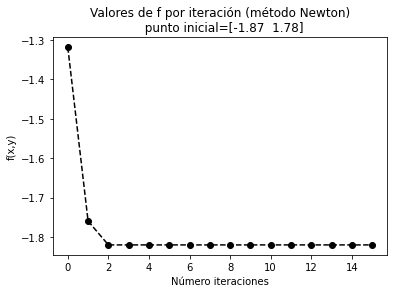
\includegraphics[width=0.63\textwidth]{images/ult_newton}
		\caption{Valores de $f$ por iteración para punto de inicio $(-1.87,1.78)$}
	\end{figure}
	Partíamos de $w_0=(-1.87,1.78)$ con $f(w_0)=-1.31841318$, tras 15 iteraciones hemos llegado al punto $\hat w = (-1.75619503, 1.76207418)$ con $f(\hat w)=-1.8200785415471565$.\\
	
	\item También podemos retomar la regresión realizada por Pseudoinversa y \textit{SGD} en el Ejercicio 2 - apartado 1. El error dentro de la muestra por Pseudoinversa era $0.07918658628900395$, el valor que al evaluarlo daba este error era $w_{lin}=(-1.11588016,-1.24859546,-0.49753165)$. Y mediante \textit{SGD} estimábamos error $0.0816898877496507$, el valor que al evaluarlo daba este error era $\hat w=(-1.24069346, -0.17997056, -0.46016084)$. Intentaremos mejorar el resultado obtenido mediante $\textit{SGD}$.
	
	\textit{Nota:} necesitaremos la matriz Hessiana, pero no es complicado calcularla,
	$$\nabla ^2 E_{in}(w)= \frac{\partial}{\partial w} \left(\frac{2}{N}(X^TXw-X^Ty)\right)=\frac{2}{N}X^TX$$

	Si aplicamos el método de Newton para punto inicial $\hat w$, con 15 iteraciones obtenemos la gráfica
	\begin{figure}[H]
		\centering
		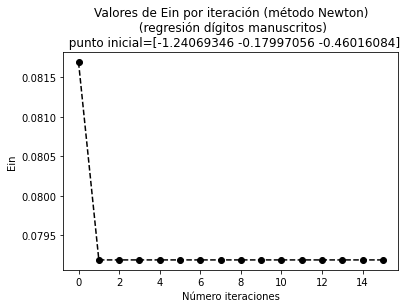
\includegraphics[width=0.63\textwidth]{images/newton_digitos_manus}
		\caption{Valores de $E_{in}$ por iteración para punto de inicio $\hat w$}
	\end{figure}
	y llegamos a $\tilde w=(-1.11588016, -1.24859546, -0.49753165)$ con $E_{in}(\tilde w)=0.07918658628900395$, que es el óptimo.
	
	La aplicación, posterior a \textit{SGD}, del método de Newton ha funcionado para mejorar el error que obteníamos solamente mediante \textit{SGD}.
	\end{itemize}
\end{document}
	

